\documentclass[11pt]{article}
\usepackage{amsmath,amssymb,amsfonts}
\usepackage{geometry}
\geometry{margin=1in}
\usepackage{graphicx}
\usepackage{booktabs}
\usepackage{natbib}
\bibliographystyle{plainnat}

\newcommand{\bxi}{\boldsymbol{\xi}}
\newcommand{\bx}{\mathbf{x}}
\newcommand{\avg}[1]{\langle #1 \rangle}

\title{Gaussian vs Exact Alignment Distribution for the LSE Phase Boundary}
\author{}
\date{}

\begin{document}
\maketitle

\section{The two phase boundaries}

The LSE energy on the $N$-sphere $|\bx|^2 = N$ is
\begin{equation}
H_{\mathrm{LSE}}(\bx) = -\frac{1}{\beta_{\mathrm{net}}}\ln\left(\sum_{\mu=1}^{M}\exp\!\big(\beta_{\mathrm{net}}\,\bxi^\mu\!\cdot\!\bx\big)\right),
\label{eq:lse}
\end{equation}
with $M = e^{\alpha N}$ patterns drawn uniformly on $S^{N-1}(\!\sqrt{N})$ and $\beta_{\mathrm{net}}$ the kernel inverse variance.  In~\citep{icml2026theory}, the retrieval equilibrium overlap is (Eq.~33)
\begin{equation}
\phi_{\mathrm{LSE}}(T) = \tfrac{1}{2}\!\left[-T + \sqrt{T^2 + 4}\right],
\label{eq:phi_eq}
\end{equation}
and the retrieval free energy density is (Eq.~34)
\begin{equation}
f_{\mathrm{ret}}(T) = 1 - \phi_{\mathrm{LSE}}(T) - \frac{T}{2}\ln\!\big(1-\phi_{\mathrm{LSE}}^2(T)\big)\,.
\label{eq:f_ret}
\end{equation}
These depend only on the single-pattern energy $u_{\mathrm{LSE}}(\phi) = 1-\phi$ and the geometric entropy $s(\phi) = \tfrac{1}{2}\ln(1-\phi^2)$; they do not involve the alignment distribution and are exact.

The phase boundary $\alpha_c(T)$ is determined by setting $f_{\mathrm{ret}}(T) = u_{\mathrm{noise}}(\alpha)$ (Eq.~22 of~\citep{icml2026theory}).  The noise floor energy $u_{\mathrm{noise}} = 1 - \varphi_{\max}$ depends on the maximum spurious alignment $\varphi_{\max}$, which in turn depends on the alignment distribution.

\paragraph{Gaussian approximation.}
Using the Gaussian density $f(\phi) \propto e^{-N\phi^2/2}$ (Eq.~23 of~\citep{icml2026theory}):
\begin{equation}
\varphi_{\max}^{\mathrm{Gauss}} = \sqrt{2\alpha}\,,\qquad
u_{\mathrm{noise}}^{\mathrm{Gauss}} = 1 - \sqrt{2\alpha}\,,\qquad
\alpha_c^{\mathrm{Gauss}}(T) = \tfrac{1}{2}\!\big(1 - f_{\mathrm{ret}}(T)\big)^2\,.
\label{eq:gauss}
\end{equation}
At $T = 0$: $f_{\mathrm{ret}} = 0$, giving $\alpha_c^{\mathrm{Gauss}}(0) = 0.5$.

\paragraph{Exact spherical density.}
Using the exact density $f(\phi) = C_N(1-\phi^2)^{(N-3)/2}$ on the sphere:
\begin{equation}
\varphi_{\max}^{\mathrm{exact}} = \sqrt{1-e^{-2\alpha}}\,,\qquad
u_{\mathrm{noise}}^{\mathrm{exact}} = 1 - \sqrt{1-e^{-2\alpha}}\,,\qquad
\alpha_c^{\mathrm{exact}}(T) = -\tfrac{1}{2}\ln\!\Big(1 - \big(1 - f_{\mathrm{ret}}(T)\big)^2\Big)\,.
\label{eq:exact}
\end{equation}
At $T = 0$: $f_{\mathrm{ret}} = 0$, giving $\alpha_c^{\mathrm{exact}}(0) = -\tfrac{1}{2}\ln(0) = \infty$.  The exact density vanishes at $|\phi| = 1$, so no finite $\alpha$ produces a pattern at overlap~1.

\paragraph{Comparison.}
Table~\ref{tab:compare} compares the two boundaries at selected temperatures.

\begin{table}[h]
\centering
\caption{Phase boundary $\alpha_c(T)$ for LSE under Gaussian and exact alignment distributions.}
\label{tab:compare}
\begin{tabular}{ccccc}
\toprule
$T$ & $\phi_{\mathrm{eq}}$ & $f_{\mathrm{ret}}$ & $\alpha_c^{\mathrm{Gauss}}$ & $\alpha_c^{\mathrm{exact}}$ \\
\midrule
0.001 & 0.9995 & 0.004 & 0.496 & 2.42 \\
0.10  & 0.951  & 0.166 & 0.348 & 0.594 \\
0.30  & 0.861  & 0.342 & 0.217 & 0.284 \\
0.50  & 0.781  & 0.454 & 0.149 & 0.177 \\
1.00  & 0.618  & 0.623 & 0.071 & 0.077 \\
2.00  & 0.414  & 0.774 & 0.026 & 0.026 \\
\bottomrule
\end{tabular}
\end{table}

The two curves agree to within $\sim$3\% for $T > 1.5$ and diverge at low $T$: at $T = 0.1$ the exact boundary is 71\% higher.  The question is which curve the Monte Carlo data follow.

\begin{figure}[t]
\centering
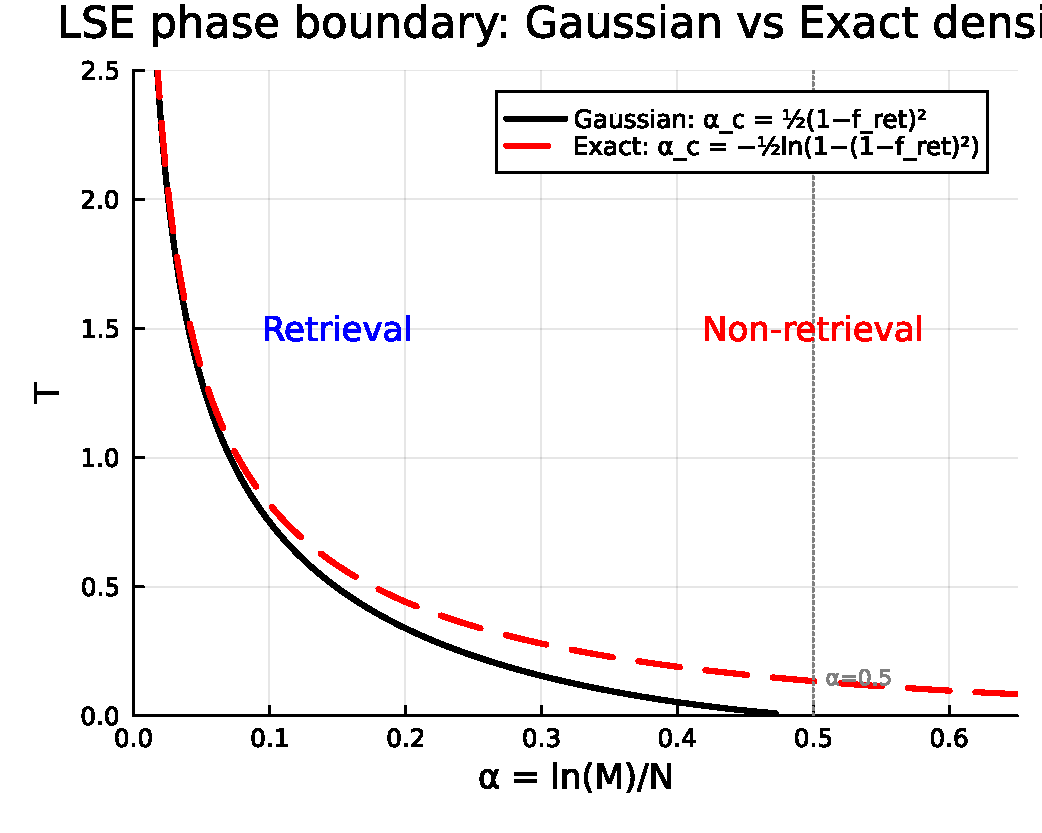
\includegraphics[width=0.7\textwidth]{../code/panels_LSE/phase_boundary_comparison.pdf}
\caption{LSE phase boundary $\alpha_c(T)$: Gaussian (solid black) vs exact (dashed red).  The two agree at high~$T$ and diverge at low~$T$.  MC data points (to be added) will distinguish the two.}
\label{fig:phase_boundary}
\end{figure}

\section{Monte Carlo test}

To distinguish the two predictions, we run the v8m-style Monte Carlo protocol with the LSE energy~\eqref{eq:lse}.  The simulation parameters and results will be reported here after completion.

\bibliography{references}

\end{document}
